\documentclass[twocolumn,apj,numberedappendix,appendixfloats]{openjournal}
% Available options:
% [twocolumn] - two-column mode
% [onecolumn] - (default) main text in one-column mode
% [apj]       - typeset in the style of ApJ.
% [apjl]      - (default) typeset in the style of ApJ Letters 
% [tighten]   - some adjustments to approximate grid typesetting
% [numberedappendix]   - number appendix sections as A, B, etc
% [appendixfloats]  - use separate numbering for floats within appendix
% [twocolappendix]  - make appendix in two-col mode in a two-col paper


%%%%% PACKAGES %%%%%
% Optional useful packages
\usepackage{newtxtext,newtxmath,amsmath}
\usepackage[T1]{fontenc}
\usepackage{graphicx}
\usepackage{enumitem}
\usepackage{xcolor}
\usepackage{hyperref}
\usepackage{gensymb}
\usepackage{CJK}
\usepackage{tabularx}
\usepackage{orcidlink}
\hypersetup{
    unicode, 
    colorlinks=true,
    linkcolor=linkcolor,
    citecolor=linkcolor,
    filecolor=linkcolor,
    urlcolor=linkcolor,
}
\definecolor{linkcolor}{rgb}{0.0,0.3,0.5}


% \usepackage{newtxtext,newtxmath,amsmath}
% \usepackage{xcolor}
% \usepackage{textgreek}
% \usepackage[utf8]{inputenc}
% \usepackage[english]{babel}
% \usepackage{hyperref}
% \hypersetup{
%     unicode, 
%     colorlinks=true,
%     linkcolor=linkcolor,
%     citecolor=linkcolor,
%     filecolor=linkcolor,
%     urlcolor=linkcolor,
% }
% \usepackage{color,colortbl}
% \definecolor{linkcolor}{rgb}{0.0,0.3,0.5}
% \usepackage{orcidlink}

%%%%% COMMANDS %%%%%
% Optional useful commands

% I use the following command to indicate comments with \SB{My comment here}.
% Before submission, you should comment this \newcommand out,
% to make sure you do not have any leftover comments!
\newcommand{\SB}[1]{{\textcolor{purple}{SB: #1}}}
\newcommand{\comment}[1]{\textcolor{lightgray}{#1}}

%%%%%%%%%%%%%%%%%%%%%%%%%%%%%%%%%%%%%%%%%%%%%%%%%
%%%%%%%%%%%%%%%%%%%%%%%%%%%%%%%%%%%%%%%%%%%%%%%%%
\begin{document}
\title{Reading Between the Residuals: Hidden Physics in Stellar Spectral Mismatches}

\author{\vspace{-1.5cm}Sven Buder$^{1,*}$\orcidlink{0000-0002-4031-8553}}
\author{David W. Hogg$^{2,3,4}$\orcidlink{0000-0002-4031-8553}}

% \affiliation{$^{1}$Research School of Astronomy and Astrophysics, Australian National University, Canberra, ACT 2611, Australia}
% \affiliation{$^{2}$Center for Computational Astrophysics, Flatiron Institute, 162 Fifth Avenue, New York, NY 10010, USA}
% \affiliation{$^{3}$Max-Planck-Institut für Astronomie, Königstuhl 17, D-69117 Heidelberg, Germany}
% \affiliation{$^{4}$Center for Cosmology and Particle Physics, Department of Physics, New York University, 726 Broadway, New York, NY 10003, USA}



\thanks{E-mail: sven.buder@anu.edu.au}
\thanks{$^*$Australian Research Council DECRA Fellow}

\begin{abstract}
We investigate the diagnostic power of spectral residuals—the difference between observed stellar spectra and synthetic models—as a source of information on stellar and interstellar phenomena not captured by current spectral synthesis. By fitting a data-driven model to these residuals, we demonstrate that fundamental stellar parameters can be recovered to surprising precision ($\Delta T_\mathrm{eff} < 350\,\mathrm{K}$, $\Delta \log g < 0.4$, and $\Delta\mathrm{[Fe/H]} < 0.1$), indicating that significant parameter-dependent structure remains in the residuals. This unmodelled information likely includes physical effects such as 3-dimensional atmosphere effects (not covered by 1-dimensional synthesis), stellar activity (e.g. linked to X-ray luminosity or indices like $\log R_{HK}$), and interstellar absorption features like diffuse interstellar bands (DIBs) and KI lines. We show that aligning spectra to the interstellar velocity frame or using extinction as a proxy for ISM density allows us to isolate and learn characteristic templates for these features. Analogous to binary decomposition, this residual fitting approach offers a new avenue to template peculiar spectral signatures—such as Balmer line core asymmetries due to 3D effects or proxies for chromospheric activity—even in the absence of direct spectral indicators like the Ca H\&K lines. Our method opens new prospects for inferring stellar properties from spectral features currently not covered by synthesis.
\end{abstract}

% Write your keywords here
\begin{keywords}
    {}%{Choose up to 6 keywords from \href{https://academic.oup.com/DocumentLibrary/mnras/keywords.pdf}{here} and write them like: keyword1 -- keyword2.}
\end{keywords}

\maketitle

% \section{Introduction}
% \label{sec:introduction}

% The paper is structured as follows: Section~\ref{sec:data} describes the data of \dots. Section~\ref{sec:analysis} analyses \dots. We discuss our analysis in the context of our hypotheses in Section~\ref{sec:discussion} and bundles our results into an overarching conclusion in Section~\ref{sec:conclusions}.

%%%%%%%%%%%%%%%%%%%%%%%%%%%%%%%%%%%%%%%%%%%%%%%%%
%%%%%%%%%%%%%%%%%%%%%%%%%%%%%%%%%%%%%%%%%%%%%%%%%
\section{Data} \label{sec:data}

For this analysis, we use the observed and best-fit model spectra as well as labels from GALAH DR4 \citep{Buder2025b}.

\subsection{Stellar Labels} \label{sec:data_labels}

For this pilot project, we select spectra of 7511 stars that were observed between 10 and 12 July 2017 with \texttt{flag\_sp} < 2048 in GALAH DR4, that is, with sufficient spectral quality (SNR > 10) and estimated stellar parameters. We explicitly do not cut out stars with emission lines or binary signatures.

For our first test to of overall line modelling imperfections across different stellar types, we simply use the three main stellar parameters as input:
\begin{equation}
    l \in [T_\mathrm{eff}, \log g, \mathrm{[Fe/H]}] \label{eq:tlf}
\end{equation}

We plot the their distribution in Fig.~\ref{fig:labels_teff_logg_feh}.

\begin{figure}
    \centering
    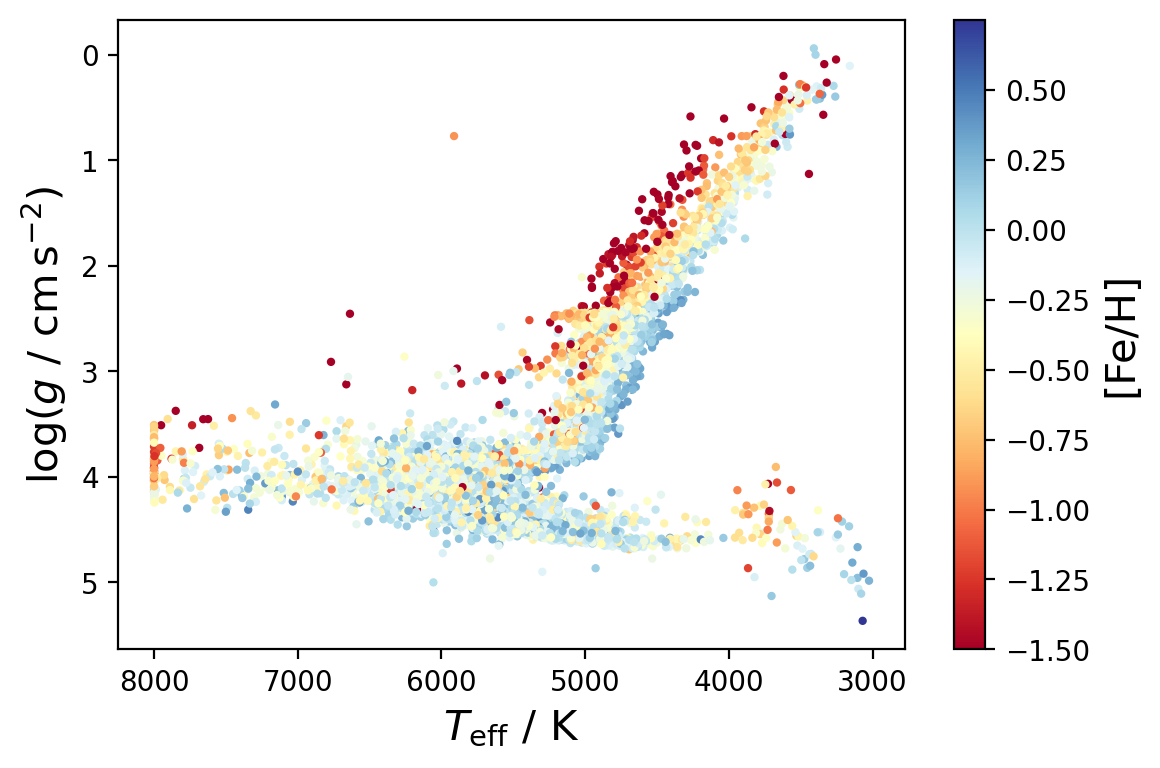
\includegraphics[width=\columnwidth]{figures/labels_teff_logg_feh.png}
    \caption{Stellar parameters ($T_\mathrm{eff}$ vs. $\log g$, colored by $\mathrm{[Fe/H]})$ of the subset of GALAH DR4 used for this analysis.}
    \label{fig:labels_teff_logg_feh}
\end{figure}

\SB{Could also be $\log R_{HK}$ or X-ray luminosity or extinction? -> check draft on Hyades analysis, where we have those!}

\subsection{Residual spectra} \label{sec:data_residuals}

Because spectra are reported in their native pixel grid (with a wavelength solution fitted to it) in GALAH DR4, but a model has to be built with a shared wavelength grid, we first interpolated all spectra onto the same wavelength grid.

To do this, for each CCD we identified the highest first pixel wavelength, the median dispersion across all spectra, and the lowest last pixel wavelength. For CCDs 1-4, this resulted in a common wavelength grid of $4719.0299..0.046..4893.8808$, $5655.5298..0.0547..5863.0182$, $6486.0104..0.0631..6726.4572$, and 
$7689.1261..0.0735..7874.3127$\,\AA.s We then use the \textsc{numpy.interpolate} routine to interpolate a spectra onto the same wavelength grid.

The final result are two matrices of 5711 stars with 13927 pixels with either flux residuals of observed minus synthetic flux (\texttt{sob - smod}) as well as the inverse variance of the observed uncertainty ($1/\texttt{uob}^2$).

%%%%%%%%%%%%%%%%%%%%%%%%%%%%%%%%%%%%%%%%%%%%%%%%%
%%%%%%%%%%%%%%%%%%%%%%%%%%%%%%%%%%%%%%%%%%%%%%%%%
\section{Analysis} \label{sec:analysis}

We use \textit{The Cannon} \citep{Ness2015} in its version 2 by \citet{Casey2016}.

\subsection{Test 1: Predicting residuals with Stellar Parameters}

\begin{figure*}
    \centering
    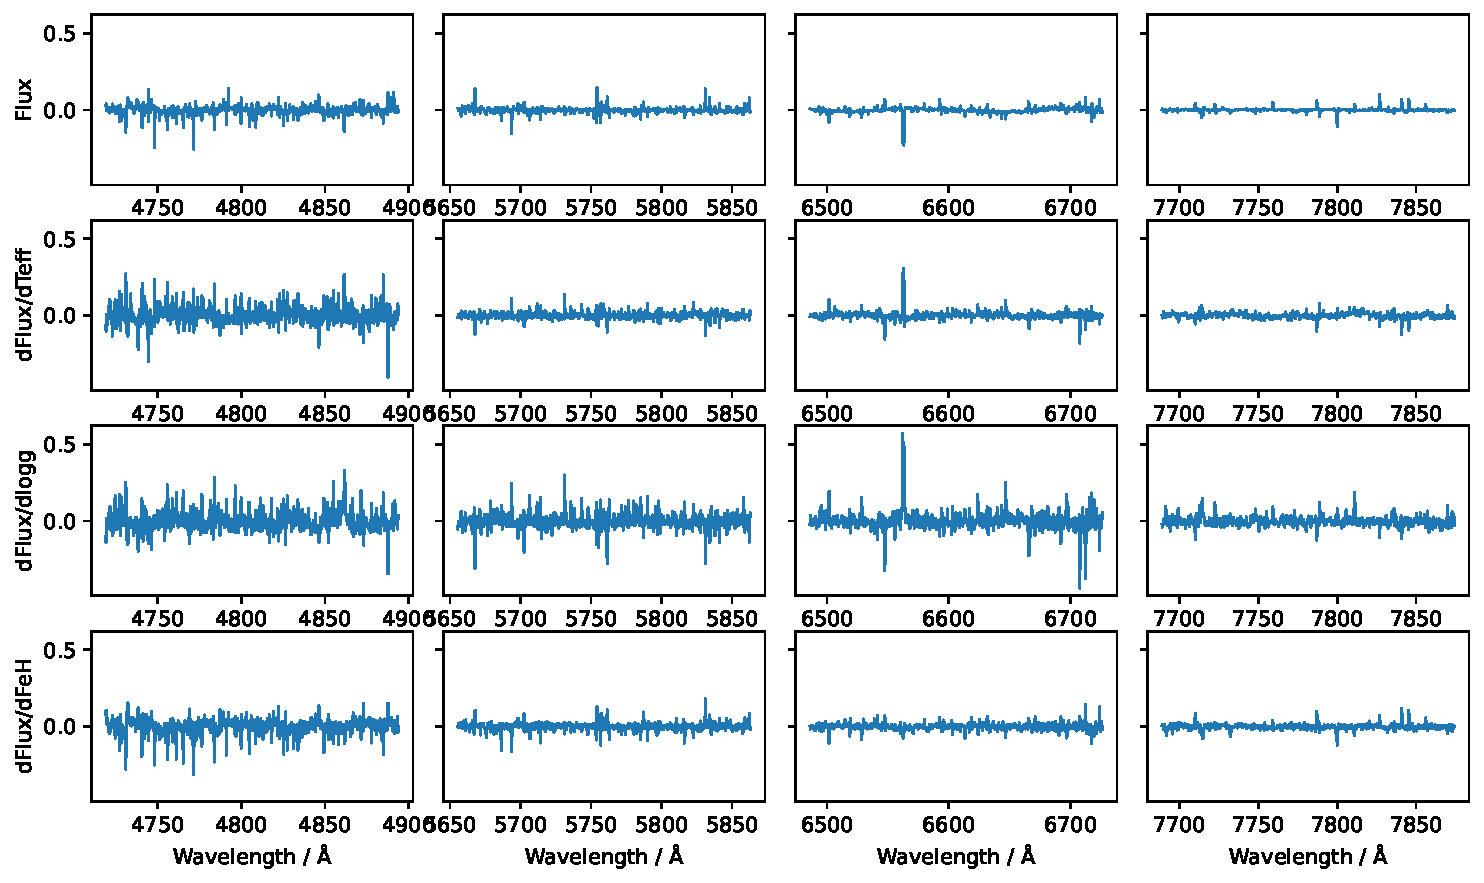
\includegraphics[width=\textwidth]{figures/tc_res_tlf_theta.pdf}
    \caption{Median Residual and linear coefficients.}
    \label{fig:tc_res_tlf_theta}
\end{figure*}

In our first test, we build a quadratic model with \textit{The Cannon} that predicts the residual flux \texttt{sob - smod} of GALAH DR4 based on the stellar label from Eq.~\ref{eq:tlf}. We show the median residual spectrum as well as the linear coefficients that \textit{The Cannon} estimates for the change of residual flux with labels in Fig.~\ref{fig:tc_res_tlf_theta}. While the majority of the residual spectrum are close to 0, the HI Balmer lines (in particular Halpha at 6563\,\AA) stick out. These lines are usually not well fitted with 1D synthesis tools and have thus also been masked out in the fitting of GALAH DR4.

\SB{point out features in Fig.~\ref{fig:tc_res_tlf_theta}}.

Once the model is trained, we use it to recover the labels that it was trained on. Here we would expect very bad recovery performance, if the spectra are actually well fitted within the uncertainties, and the residuals of the spectra represent the underlying spectrum noise.

\begin{figure*}
    \centering
    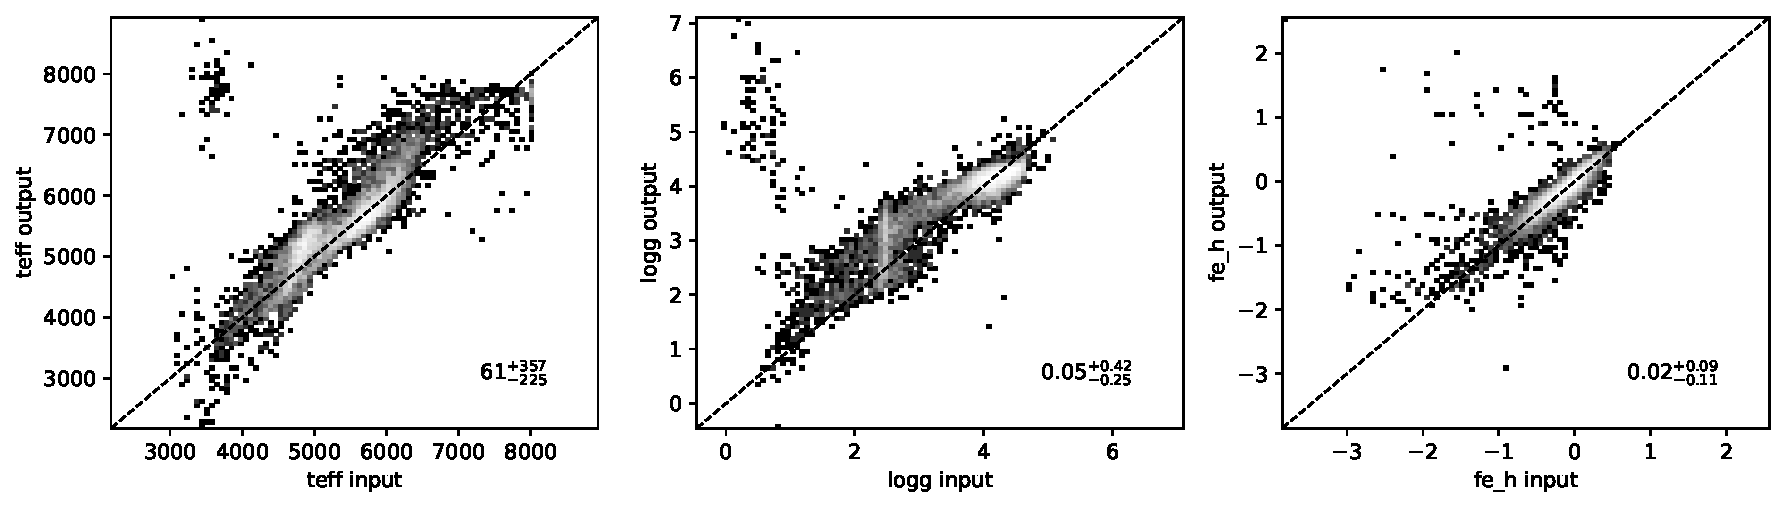
\includegraphics[width=\textwidth]{figures/tc_res_tlf_recovery.pdf}
    \caption{Recovery of labels: output (y-axis) vs. input.}
    \label{fig:tc_res_tlf_recovery}
\end{figure*}

When looking at Fig.~\ref{fig:tc_res_tlf_recovery} with training and recovered labels on x-axis and y-axis, respectively, we see that a considerable amount of information on stellar parameters must have remained in the residual spectra. \textit{The Cannon} is recovery is close to a one-to-one relation for all three labels, with only small biases and surprisingly small scatters of $\Delta T_\mathrm{eff} < 350\,\mathrm{K}$, $\Delta \log g < 0.4$, and $\Delta\mathrm{[Fe/H]} < 0.1$.

Some insights from looking at individual spectra:
\begin{itemize}
    \item Fig.~\ref{fig:residuals_170711005801103}: Balmer lines fit well by \textit{The Cannon} model. Several regions with strong residual lines (e.g. 4748, 4773, 5695, 5755, 7800) indicate that some lines were not predicted well by the spectrum synthesis, but can be fitted well with a data-driven model. These lines indicate imperfect line synthesis. Some sharp outliers remain, e.g. 4735 or 7705, and are likely true pixel outliers.
    \item Fig.~\ref{fig:residuals_170711005801334}: More residuals can be seen, especially in CCD1, which are again can be recovered by the data-driven model, and hint at imperfect spectrum synthesis. Strong residuals for several lines beyond 7800 remain -> remember talk from Kathryn Kreckel on emission lines.
    \item Fig.~\ref{fig:residuals_170712003101121}: An overall stronger residual remains in CCD1, but can also not really be recovered by The Cannon model. This is equally true for some strong features at 5780, 5797, 6613, and 7699 -- all known interstellar features which should not be fitted well based on stellar labels.
\end{itemize}

\begin{figure*}
    \centering
    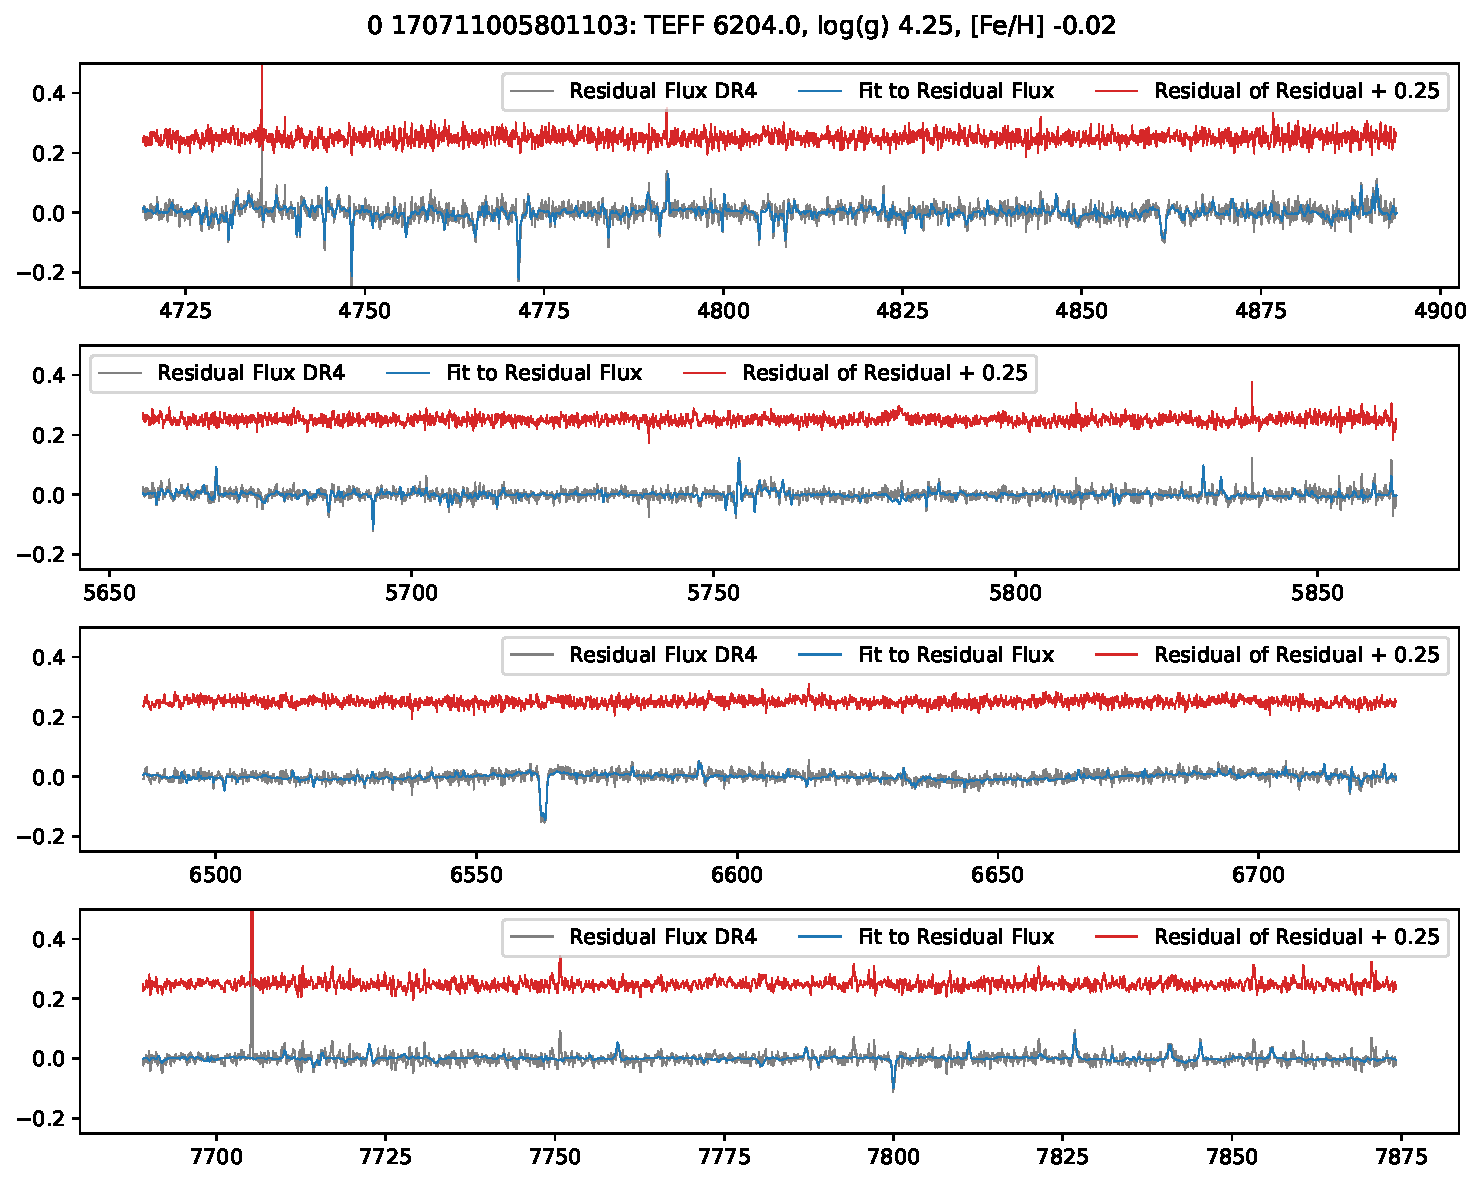
\includegraphics[width=\textwidth]{figures/residuals_170711005801103.pdf}
    \caption{Residual spectra (black), fits to these residua (blue), and residuals of the residua (red) for 170711005801103.}
    \label{fig:residuals_170711005801103}
\end{figure*}

\begin{figure*}
    \centering
    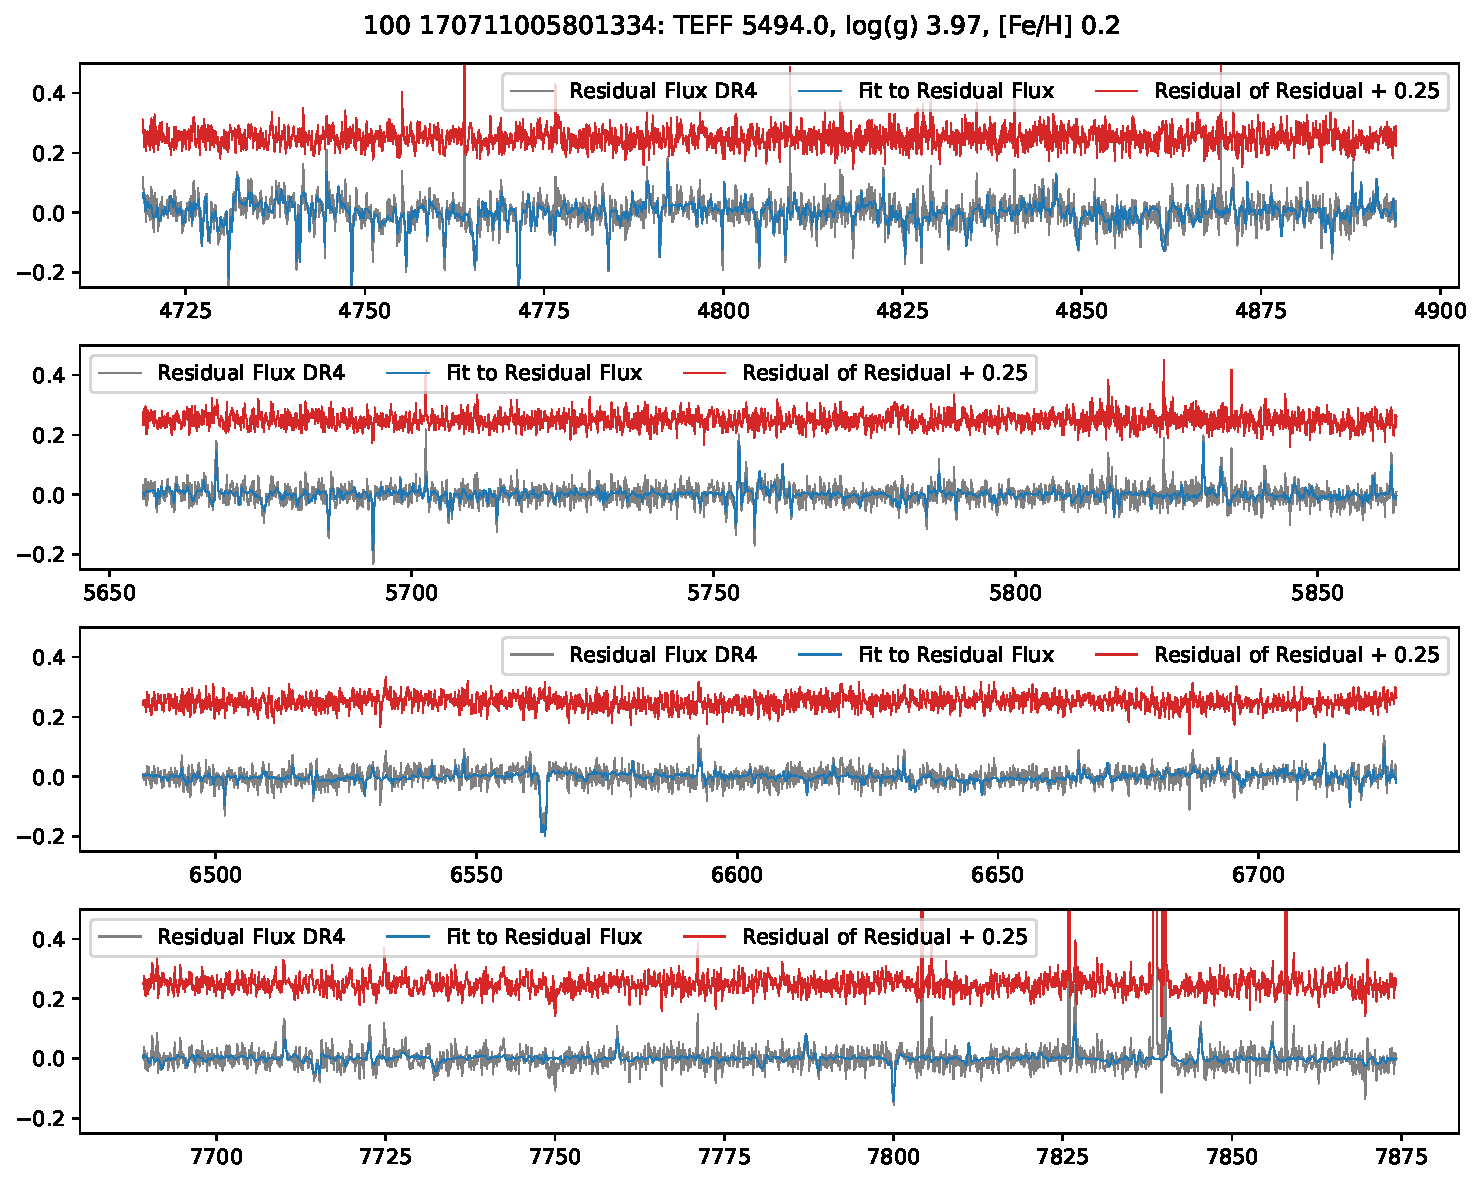
\includegraphics[width=\textwidth]{figures/residuals_170711005801334.pdf}
    \caption{Residual spectra (black), fits to these residua (blue), and residuals of the residua (red) for 170711005801334.}
    \label{fig:residuals_170711005801334}
\end{figure*}

\begin{figure*}
    \centering
    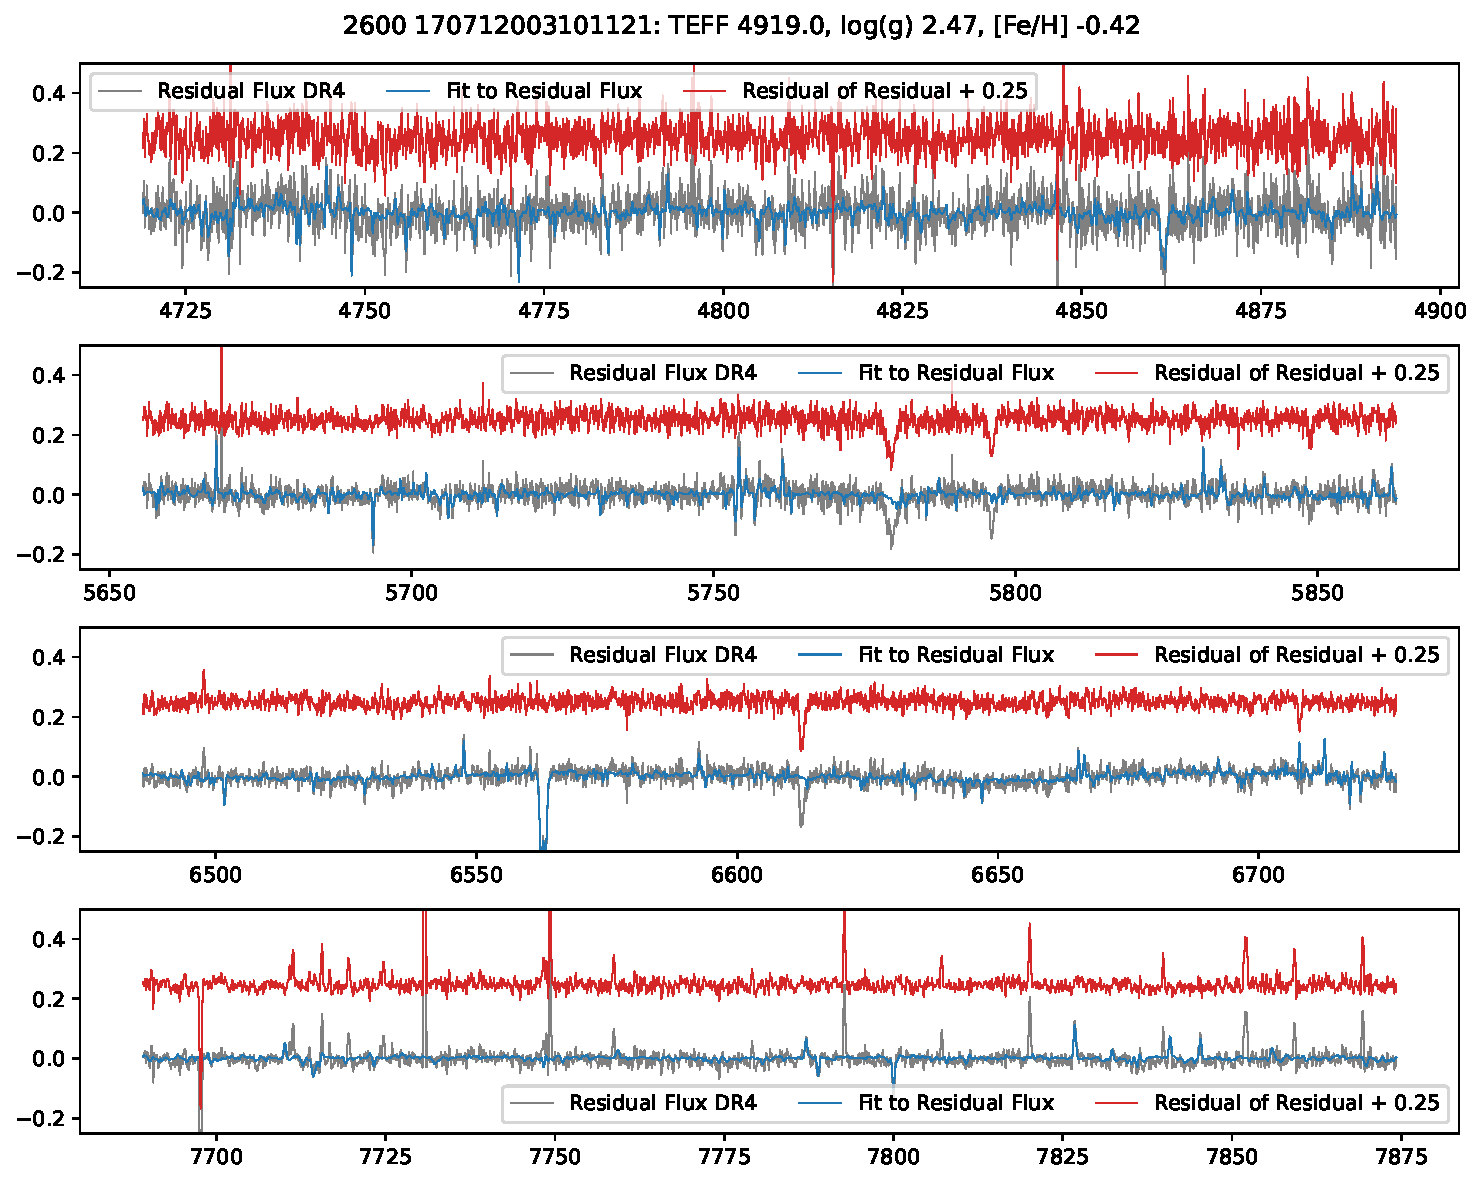
\includegraphics[width=\textwidth]{figures/residuals_170712003101121.pdf}
    \caption{Residual spectra (black), fits to these residua (blue), and residuals of the residua (red) for 170712003101121.}
    \label{fig:residuals_170712003101121}
\end{figure*}

\subsection{Test 2: Predicting activity with logRHK or X-ray luminosity}

\SB{see research on GALAH DR4 observations of Hyades with Xlum correlating to [Fe/H].}

\subsection{Test 3: Predicting ISM density with extinction}

\SB{Remember Fig.~\ref{fig:residuals_170712003101121}, where ISM features were strong in residuals. Could use template by \citet{Vogrincic2023} to actually fit ISM column density and radial velocity at the time and overcome degeneracies like stellar and interstellar KI lines.}

%%%%%%%%%%%%%%%%%%%%%%%%%%%%%%%%%%%%%%%%%%%%%%%%%
%%%%%%%%%%%%%%%%%%%%%%%%%%%%%%%%%%%%%%%%%%%%%%%%%
\section{Discussion} \label{sec:discussion}

%%%%%%%%%%%%%%%%%%%%%%%%%%%%%%%%%%%%%%%%%%%%%%%%%
%%%%%%%%%%%%%%%%%%%%%%%%%%%%%%%%%%%%%%%%%%%%%%%%%
\section{Conclusions} \label{sec:conclusions}


%%%%%%%%%%%%%%%%%%%%%%%%%%%%%%%%%%%%%%%%%%%%%%%%%
%%%%%%%%%%%%%%%%%%%%%%%%%%%%%%%%%%%%%%%%%%%%%%%%%
% \section*{Acknowledgments}

% We acknowledge the traditional owners of the land on which the ANU stands, the Ngunnawal and Ngambri people. We pay our respects to elders past, and present and are proud to continue their tradition of surveying the night sky and its mysteries to better understand our Universe.

% SB acknowledges support from the Australian Research Council under grant numbers DE240100150.

%%%%%%%%%%%%%%%%%%%%%%%%%%%%%%%%%%%%%%%%%%%%%%%%%
%%%%%%%%%%%%%%%%%%%%%%%%%%%%%%%%%%%%%%%%%%%%%%%%%
\section*{Data Availability}

All code to reproduce the analysis and figures can be publicly accessed via \url{https://github.com/svenbuder/residual_cannon}.

%%%%%%%%%%%%%%%%%%%%%%%%%%%%%%%%%%%%%%%%%%%%%%%%%
%%%%%%%%%%%%%%%%%%%%%%%%%%%%%%%%%%%%%%%%%%%%%%%%%
\bibliographystyle{mnras}
\bibliography{bib}

%%%%%%%%%%%%%%%%%%%%%%%%%%%%%%%%%%%%%%%%%%%%%%%%%
%%%%%%%%%%%%%%%%%%%%%%%%%%%%%%%%%%%%%%%%%%%%%%%%%
%\begin{appendix}

%\section{Interesting information that is not vital for the main story of your paper}

%\end{appendix}

\end{document}